\documentclass[a4paper,11pt]{article}
\usepackage[utf8]{inputenc}
\usepackage[spanish]{babel}
\usepackage{amsmath}%paquete matemático
\usepackage{amsfonts}% proporciona caracteres para ciertos conjuntos matematicos
\usepackage{eurosym}% paquete para simbolo euro
\usepackage[pdftex]{graphicx}%para insertar figuras .png o .jpg
\usepackage{multirow}% crea varias tablas en el que el texto ocupe varias filas
\usepackage{float}
%\parindent=20px
\begin{document}
   \part{Ecuación}
  $\sum \binom{a}{b}=(n+1)!-1$
   \part{Imagen}
\begin{figure}[!h]
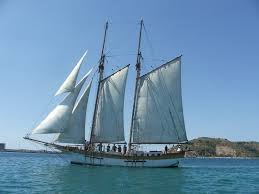
\includegraphics[scale=.75]{indice.jpg} %ruta de la página
\caption{Foto}%% pie de pagina
\label{fig:indice.jpg}
\end{figure}
\part{tabla}
\begin{center}
\begin{tabular}{|c|c|c|c|}
\hline Celda 1 & Celda 2 & Celda 3 & Celda 4 \\
\hline Celdas 5 & Celda 6 & Celda 7 & Celda 8 \\
\hline Celda 9 & Celda 10 & Celda 11 & Celda 12\\
\hline Celda 13 & \multicolumn{3}{|c|}{Celda 15 y Celda 16}\\
\hline
\end{tabular}
\end{center}
\bibliography{biblioteca}
\nocite{*}
%\cite[informacion adicional a añadir]{cita1}

\bibliographystyle{plain}
\end{document}
